\documentclass[11pt,a4paper]{article}
\usepackage[T1]{fontenc}
\usepackage{lmodern,microtype,amsmath,amssymb,amsthm,mathtools,mathrsfs}
\usepackage[margin=25mm,headheight=14pt]{geometry}
\usepackage{graphicx,xcolor,booktabs,tabularx,longtable,enumitem}
\usepackage{tikz,pgfplots}
\usetikzlibrary{arrows.meta,positioning,calc,fit,backgrounds}
\pgfplotsset{compat=1.18}
\usepackage{fancyhdr}
\usepackage[colorlinks=true,linkcolor=teal!60!black,citecolor=teal!60!black,urlcolor=blue!55!black]{hyperref}
\hypersetup{pdftitle={Positive Cut-Word Models for the Kanade-Russell I1 Bijection Problem},pdfauthor={Christopher Yamba},pdfsubject={General positive divided differences, partial KR1 constructions, and Lean certificates}}
\definecolor{ink}{HTML}{17334A}
\definecolor{teal}{HTML}{087F8C}
\definecolor{gold}{HTML}{C58A28}
\definecolor{pale}{HTML}{EFF6F7}
\definecolor{warn}{HTML}{A43D35}
\pagestyle{fancy}
\fancyhf{}
\lhead{\small\textcolor{ink}{Yamba AI Math}}
\rhead{\small KR1: positive models and the remaining bridge}
\cfoot{\thepage}
\setlength{\parskip}{5pt}
\setlength{\parindent}{0pt}
\setlist{itemsep=3pt,topsep=5pt}
\newtheorem{theorem}{Theorem}[section]
\newtheorem{lemma}[theorem]{Lemma}
\newtheorem{corollary}[theorem]{Corollary}
\newtheorem{proposition}[theorem]{Proposition}
\theoremstyle{definition}
\newtheorem{definition}[theorem]{Definition}
\newtheorem{example}[theorem]{Example}
\newcommand{\wt}{\operatorname{wt}}
\newcommand{\cm}{\operatorname{comaj}}
\newcommand{\NN}{\mathbb N}
\newcommand{\DD}{\mathcal D}
\renewcommand{\AA}{\mathcal A}
\newcommand{\BB}{\mathcal B}
\newcommand{\SSA}{\mathscr A}
\newcommand{\CC}{\mathscr C}
\newcommand{\EE}{\mathcal E}
\newcommand{\statusbox}[1]{\par\medskip\noindent\fcolorbox{teal!45}{pale}{\begin{minipage}{0.94\linewidth}#1\end{minipage}}\par\medskip}
\title{\color{ink}\LARGE Positive Cut-Word Models\\[4pt]
for the Kanade--Russell I$_1$ Bijection Problem\\[9pt]
\large A general cancellation theorem, reversible local constructions,\\
global obstructions, and supplementary Lean verification}
\author{Christopher Yamba\\[3pt]
\small Research with a GPT-6.1 Terra agent fleet\\
\small Coordinated mathematical synthesis and independent criticism}
\date{27 October 2026}

\begin{document}
\maketitle
\begin{abstract}
We investigate a structural, weight-preserving bijection for the full modulo-nine
Kanade--Russell identity KR1. The requested residue-to-gap bijection is not
obtained. The main retained result is instead a general constructive positivity
theorem for normalized divided differences. An ordered word of cuts and colored
particles converts every signed factor into a matching staircase increment.
A least-eligible sign-reversing involution works for arbitrary numbers of cuts
and markers. Applied to Xia's auxiliary product sequences, it gives explicit
positive models for all $A_n,B_n,C_n$, not merely bounded values of $n$.
We also prove a quantitative maximum-part obstruction for any injection on a
bounded-multiplicity source family, supply a reversible local bidegree surgery,
audit the existing gap-to-cluster endpoint, and retain exact failures of several
carry and recurrence recipes. Lean 4 verifies selected universal components;
the source interpretation and full word encoding have separate written review.
Novelty relative to the literature has not been established.
\end{abstract}

\statusbox{\textbf{Scope of the result.}
The all-index positive auxiliary models are proved by a written construction.
They do not yet supply the branch bijections needed to reach all KR1 gap
partitions. No weight-specific matching, ranking, or apex lookup is used to
define a claimed global map. The complete KR1 bijection remains unfinished.}

\section{The exact target and the repository baseline}

Let $\BB_N$ be the partitions of $N$ with every part congruent to
$1,3,6,8\pmod9$. Let $\AA_N$ be the ascending positive partitions
$\lambda_1\le\cdots\le\lambda_\ell$ satisfying
\begin{align}
\lambda_{i+2}-\lambda_i&\ge3,\\
\lambda_{i+1}-\lambda_i\le1&\ \Longrightarrow\
 \lambda_i+\lambda_{i+1}\equiv0\pmod3.
\end{align}
The target consists of explicit algorithms
$F:\BB_N\to\AA_N$ and $G:\AA_N\to\BB_N$, for every $N\ge0$,
with validity, weight, termination, and both inverse identities proved.

The familiar series is
\begin{equation}\label{eq:kr1}
\sum_{a,b\ge0}\frac{q^{a^2+3ab+3b^2}}
 {(q;q)_a(q^3;q^3)_b}
=\frac1{(q,q^3,q^6,q^8;q^9)_\infty}.
\end{equation}
Here $(z;q)_r=\prod_{j=0}^{r-1}(1-zq^j)$. Kur\c{s}ung\"oz's
cluster construction identifies the sum with the gap class \cite{kursungoz}.
Xia and Mizuno give recent analytic treatments \cite{xia,mizuno}.
The Palomar record for Mizuno's formalization reports Lean and independent
nanoda checking of the three symmetric identities at a pinned source revision
\cite{palomar}. We inspected the registry metadata, pinned challenge statement,
and solution wrapper, but did not locally rebuild that external development.
The challenge template's placeholders are separate from the submitted solution.
An analytic or formal power-series identity is different
from the structural algorithm sought here.

The investigation starts from the corrected KR1 branch at
\texttt{4ccc4fe}, which follows PR \#15 at \texttt{2ccf9c5}.
PR \#16 proves the restricted $a=3,b=0$ sector for all its parameters and a
fixed-column-alphabet obstruction \cite{repo16}. The earlier global table
fails at weight $41$: two distinct cluster inputs share
$U=(19,12,6,3,1)$ \cite{repo15}. That failure is retained, not patched by
adding entries. The newer \texttt{watch/openai-math} branch is a source-monitoring
change and does not close KR1.

\begin{figure}[ht]
\centering
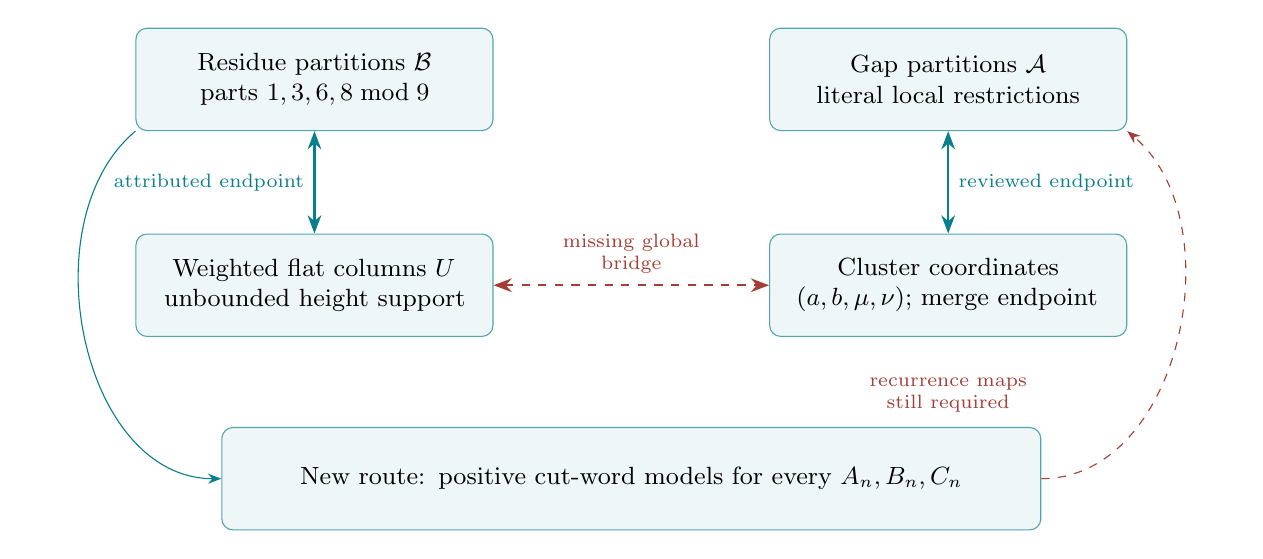
\begin{tikzpicture}[>=Stealth,node distance=13mm,
 box/.style={draw=teal!70,rounded corners,fill=pale,align=center,
 text width=43mm,minimum width=45mm,minimum height=13mm,font=\small}]
\node[box] (b) {Residue partitions $\BB$\\parts $1,3,6,8\bmod9$};
\node[box,right=35mm of b] (a) {Gap partitions $\AA$\\literal local restrictions};
\node[box,below=of b] (u) {Weighted flat columns $U$\\unbounded height support};
\node[box,below=of a] (c) {Cluster coordinates\\$(a,b,\mu,\nu)$; merge endpoint};
\draw[<->,thick,teal] (b)--node[left,font=\scriptsize]{attributed endpoint}(u);
\draw[<->,thick,teal] (a)--node[right,font=\scriptsize]{reviewed endpoint}(c);
\draw[<->,dashed,thick,warn] (u)--node[above=3pt,font=\scriptsize,align=center,fill=white,inner sep=1pt]{missing global\\bridge}(c);
\node[box,below=18mm of $(u)!0.5!(c)$,text width=100mm,minimum width=104mm] (p)
 {New route: positive cut-word models for every $A_n,B_n,C_n$};
\draw[->,teal] (b.south west) to[out=220,in=180] (p.west);
\draw[->,dashed,warn] (p.east) to[out=0,in=320] (a.south east);
\node[below=4mm of c,font=\scriptsize,align=center,text=warn]
 {recurrence maps\\still required};
\end{tikzpicture}
\caption{The full objective is unchanged. The new theorem removes signs from
all auxiliary indices, but does not complete either dashed connection.}
\end{figure}

\section{A general positive divided-difference theorem}\label{sec:main}

The construction is more general than the specific KR1 parameters.
Fix integers $d,c>0$, $n\ge0$, and $0<r_i<c$ for $0\le i\le n$.
Assume the formal nodes $z_i=q^{r_i}+q^{c-r_i}$ are distinct. Put
\[
\Phi_{d,c}(z)=\prod_{j\ge0}(1-zq^{dj}+q^{c+2dj})^{-1},
\qquad D=\Phi_{d,c}[z_0,\ldots,z_n].
\]
Divided differences have their ordinary interpolation meaning; all evaluated
expressions are interpreted coefficientwise as formal series.

\subsection{Colored cut objects}

For $n\ge1$ choose $0\le k_1\le\cdots\le k_n$, and set $k_0=0$.
Layer $i<n$ contains particles at indices
$k_i\le j\le k_{i+1}$; layer $n$ allows every $j\ge k_n$.
At each allowed cell there are independently repeatable particles
\[
\alpha_i(j): r_i+dj,\qquad \beta_i(j): c-r_i+dj.
\]
Each cut $k_i$ contributes $dk_i$ to the weight. A cell is identified by
its layer, index, and color, even when two numeric weights happen to coincide.
For $n=0$ there is one layer and no cuts.

\begin{lemma}[Cut expansion]\label{lem:cut}
The generating function of these colored cut objects is $D$.
\end{lemma}
\begin{proof}
At $z_i$, the $j$th factor splits as
$(1-q^{r_i+dj})^{-1}(1-q^{c-r_i+dj})^{-1}$.
For a finite product, the divided-difference product rule assigns the $n$
divided-difference steps, weakly in order, to factor indices
$k_1\le\cdots\le k_n$. A step at index $j$ contributes $q^{dj}$,
and each factor acquires exactly the node denominators for the layers
meeting that index. Thus it gives the displayed cells, including both endpoints
and repeated cuts. This is Xia's Lemma 2.2 \cite{xia}.
Passing to the infinite product is legitimate coefficientwise: positive
particle bases bound the number of particles, and the cut charge bounds the
cut indices whenever they are nonzero.
\end{proof}

Let $\mathcal W_n$ be all finite words with exactly $n$ separators $\mid$
and any number of letters $\alpha,\beta$. Their length is $L$.
The layer of a particle is the number of preceding separators.
Define its intrinsic weight by
\[
b(w)=\sum_{\alpha\text{ in layer }i}r_i+
      \sum_{\beta\text{ in layer }i}(c-r_i).
\]
A descent is an adjacent $\beta\alpha$ in the word; a separator interrupts
adjacency. Define
\[
\cm(w)=\sum_{\substack{1\le s<L\\w_s=\beta,\ w_{s+1}=\alpha}}(L-s).
\]

\begin{theorem}[Positive cut-word normal form]\label{thm:general}
For every $0\le m\le n$,
\begin{equation}\label{eq:general}
(q^d;q^d)_mD
 =\sum_{w\in\mathcal W_n}
 \frac{q^{b(w)+d\cm(w)}}{\prod_{h=m+1}^{L(w)}(1-q^{dh})}.
\end{equation}
Empty products have value one. The right side is the generating function of
an explicit positive family with mutually inverse word coordinates.
In particular, $(q^d;q^d)_mD\in\NN[[q]]$.
\end{theorem}

\begin{proof}
\textbf{1. Flatten the object.}
Read layer $0$, cut $1$, layer $1$, and so on. Within each layer sort particles
by index, breaking ties by $\alpha<\beta$. Record the resulting word $w$
and the index $j_t$ of every symbol, including cuts. Then
$j_1\le\cdots\le j_L$ and a strict rise occurs whenever
$w_s w_{s+1}=\beta\alpha$.

Conversely, these are the only restrictions. A weakly increasing index list
with those strict rises sorts correctly inside each layer; each particle lies
between the surrounding cut indices, inclusively. Reading the cut symbols
recovers the cuts and the layer labels. Thus flattening and decoding are
mutually inverse, including repeated equal cuts and empty layers.

\textbf{2. Subtract the forced staircase.}
If $L=0$, there are no indices or gap coordinates and every sum below is empty.
For $L>0$, proceed as follows.
Let $\epsilon_s=1$ at a descent and $0$ otherwise. Set
\[
\delta_1=j_1,\qquad
\delta_t=j_t-j_{t-1}-\epsilon_{t-1}\quad(2\le t\le L).
\]
All $\delta_t$ are nonnegative. The inverse uses cumulative sums.
The index charge is exactly
\begin{equation}\label{eq:staircase}
d\sum_{t=1}^{L}j_t
 =d\sum_{t=1}^{L}(L-t+1)\delta_t+d\cm(w).
\end{equation}
For a fixed word, independent gap coordinates therefore give denominator
$\prod_{h=1}^{L}(1-q^{dh})$.

\textbf{3. Cancel every marker jointly.}
Expand $\prod_{h=1}^{m}(1-q^{dh})$ as signed marker sets.
Marker $h$ has weight $dh$ and changes sign. Because $L\ge n\ge m$,
the coordinate $\delta_{L-h+1}$ exists and has exactly the same weight.
Select the smallest $h$ for which either its marker is present or
$\delta_{L-h+1}>0$. If marked, remove the marker and add one to that
coordinate. Otherwise insert the marker and subtract one. Earlier coordinates
stay inactive and the selected one stays active, so the same $h$ is selected
on reversal. This is a weight-preserving, sign-reversing involution.

Its fixed points have no markers and
\begin{equation}\label{eq:survivor}
\delta_{L-m+1}=\cdots=\delta_L=0.
\end{equation}
The other coordinates are free. Their generating function is
\eqref{eq:general}. For each fixed weight the signed family is finite:
positive particle bases bound $L-n$, and all coordinates have positive weight.
Cancellation therefore requires no convergence assumption beyond formal
coefficientwise finiteness.
\end{proof}

\statusbox{\textbf{What is structural here?}
The word, layer labels, and all gap coordinates are recoverable from an
individual cut object. The cancellation examines one coordinate at a time.
It neither lists partitions of the same weight nor invokes the KR1 identity.
The staircase principle is classical in character; priority for this particular
general formulation and its KR1 specialization is not claimed.}

\begin{figure}[ht]
\centering
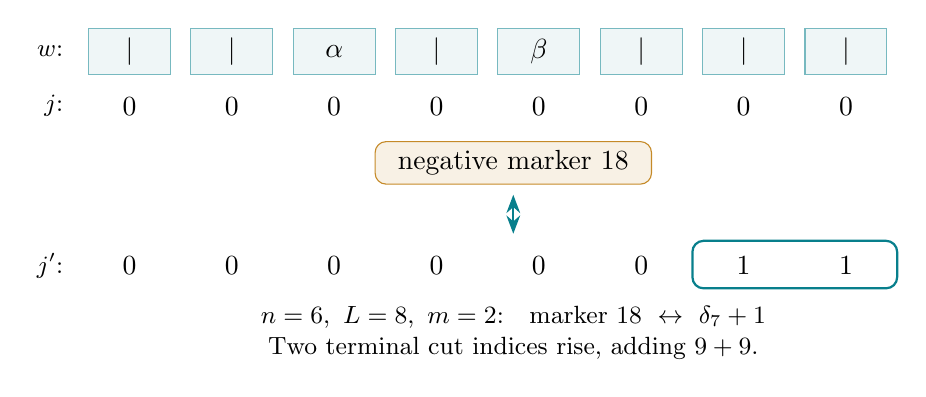
\begin{tikzpicture}[x=1.30cm,y=0.9cm,>=Stealth]
\foreach \x/\s in {0/{\mid},1/{\mid},2/{\alpha},3/{\mid},4/{\beta},5/{\mid},6/{\mid},7/{\mid}}{
 \draw[fill=pale,draw=teal!55] (\x,0) rectangle +(0.8,0.65);
 \node at (\x+0.4,0.32) {$\s$};
}
\node[anchor=east,font=\small] at (-0.15,0.32) {$w$:};
\foreach \x/\s in {0/0,1/0,2/0,3/0,4/0,5/0,6/0,7/0}
 \node at (\x+0.4,-0.45) {$\s$};
\node[anchor=east,font=\small] at (-0.15,-0.45) {$j$:};
\draw[rounded corners,fill=gold!12,draw=gold] (2.8,-1.55) rectangle (5.5,-0.95);
\node at (4.15,-1.25) {negative marker $18$};
\draw[<->,thick,teal] (4.15,-1.7)--(4.15,-2.25);
\foreach \x/\s in {0/0,1/0,2/0,3/0,4/0,5/0,6/1,7/1}
 \node at (\x+0.4,-2.7) {$\s$};
\node[anchor=east,font=\small] at (-0.15,-2.7) {$j'$:};
\draw[teal,thick,rounded corners] (5.9,-3.02) rectangle (7.9,-2.35);
\node[font=\small,align=center] at (4.15,-3.65)
 {$n=6,\ L=8,\ m=2$:\quad marker $18\ \leftrightarrow\ \delta_7+1$\\
 Two terminal cut indices rise, adding $9+9$.};
\end{tikzpicture}
\caption{A concrete joint cancellation. The intrinsic particle weights are
$28$ and $32$. Both signed partners have weight $78$.
The suffix-coordinate interpretation keeps earlier marker cancellations intact.}
\end{figure}

\subsection{A forbidden initial particle}

\begin{corollary}\label{cor:forbidden}
Multiplying the left side of \eqref{eq:general} by $(1-q^{r_0})$
also has a positive model. Replace the exponent on the right by
$b(w)+d\cm(w)+dL\epsilon_0(w)$, where $\epsilon_0(w)=1$ exactly
when the first symbol is $\alpha$; set $\epsilon_0(\varnothing)=0$.
\end{corollary}
\begin{proof}
Layer $0$, index $0$ always exists. Its $\alpha$ factor can be cancelled
directly, meaning that cell is forbidden. In a canonically ordered word,
an $\alpha$ at index $0$ in layer $0$ would necessarily be the first symbol.
Thus the exclusion is exactly $j_1\ge1$ when $w_1=\alpha$.
For a nonempty word, use $\delta_1=j_1-\epsilon_0$ instead. The empty
word has no indices, no gap coordinates, and weight zero.
Formula \eqref{eq:staircase}
acquires $dL\epsilon_0$ and the marker involution is unchanged.
\end{proof}

\noindent The restriction $m\le n$ cannot be dropped universally:
for $n=0,m=1,d=1,c=5,r_0=2$, the expression
$(1-q)/((q^2;q)_\infty(q^3;q)_\infty)$ has coefficient $-1$ at $q$.

\section{Positive models for every KR auxiliary index}

Put
\[
\EE_9=\frac1{(q^3,q^6;q^9)_\infty},\qquad
\DD_c(r_0,\ldots,r_n)=
\Phi_{9,c}[q^{r_0}+q^{c-r_0},\ldots,q^{r_n}+q^{c-r_n}].
\]
The product sequences used by Xia \cite[eqs.\ (3.5)--(3.7)]{xia} are
\begin{align}
C_n&=\EE_9(q^3;q^3)_n
 \DD_{9n+9}(3n+4,3n+7,\ldots,6n+4),\label{eq:C}\\
A_n&=\EE_9(q^3;q^3)_n(1-q^{3n-1})
 \DD_{9n}(3n-1,3n+2,\ldots,6n-1)\quad(n\ge1),\\
B_n&=C_n+q^{3n+2}A_{n+1}.
\end{align}
The separately defined $A_0$ is the KR1 product. Distinctness of the nodes
follows because equality of unequal complementary exponents would require
$3(i+j)=3n+1$ or $3n+2$, respectively.

Let $m=\lfloor n/3\rfloor$ and define the positive common tail
\[
T_n=\prod_{\substack{j>n\\3\nmid j}}(1-q^{3j})^{-1}.
\]
The essential cancellation of scalar factors is
\begin{equation}\label{eq:prefactor}
\EE_9(q^3;q^3)_n=(q^9;q^9)_m T_n.
\end{equation}
This follows by cancelling the factors with $3\nmid j$ and retaining
exactly $j=3,6,\ldots,3m$ from the numerator.

\begin{corollary}[All-index auxiliary families]\label{cor:alln}
For every $n\ge0$, $C_n$ has the positive model consisting of a common-tail
partition, a word with $n$ cuts, and nonnegative staircase coordinates with
the last $\lfloor n/3\rfloor$ coordinates zero. Its intrinsic particle bases are
\[
\alpha_i:3n+4+3i,\qquad \beta_i:6n+5-3i.
\]
For every $n\ge1$, $A_n$ has the same form with bases
\[
\alpha_i:3n-1+3i,\qquad \beta_i:6n+1-3i,
\]
and the initial $\alpha$ exclusion in Corollary~\ref{cor:forbidden}.
$B_n$ is the indicated disjoint union with a fixed weight shift.
\end{corollary}
\begin{proof}
Apply Theorem~\ref{thm:general}, Corollary~\ref{cor:forbidden}, and
\eqref{eq:prefactor}. All bases are positive. The assertion needs only
the cut expansion and the displayed definitions; it does not assume
the analytic KR1 evaluation or the three-state recurrence.
\end{proof}

\subsection{Why treating each cut separately fails}

At the all-zero cut tuple, the $C_n$ summand has coefficient $-1$ at
$q^9$ for every $n\ge3$. Indeed, the residual marker product contains
$(1-q^9)$, while every remaining common or node particle has weight
strictly greater than $9$. There is no positive weight-$9$ particle to
cancel that term inside the fixed cut.

This rules out a positive construction that preserves every cut tuple.
It does not rule out positivity of the sum. For $n=3$, increasing the last
empty cut introduces charge $9$. With particles present, a simple cut shift
can remove an occupied boundary cell. The staircase construction handles
both cases: its suffix increments move whichever mixture of cuts and particles
is actually present. It also avoids the failure of cancelling a $q^{18}$
marker by shifting one particle twice after a $q^9$ cancellation. Such a shift
can re-enter a previously cancelled image; the joint least-coordinate rule
preserves the already inactive coordinates.

\subsection{An exact finite check, with its limits}

The independent program \texttt{positive\_coefficients.py} builds the positive
word series directly (with $A_0$ separately implemented as its defining product)
and compares it with a literal last-two-parts gap
recursion. For $0\le n\le8$, $A_n$ agrees with minimum-part bound $3n+1$
and $C_n$ with bound $3n+3$, through weight $45$, except that the explicitly
costlier $A_1$ word traversal is capped at $30$. All comparisons agree.
There are $813$ checked coefficients across these eighteen comparisons.
This validates the transcription, especially the initial descent condition;
it does not supply a bijection between these families.

\section{The missing recurrence bijections}\label{sec:gap}

The gap side has a direct three-state branching description. With
$x=3n+1$, $y=3n+2$, $z=3n+3$, its transfer matrix is
\begin{equation}\label{eq:matrix}
M_n=
\begin{pmatrix}
(1+q^x)(1+q^y)&q^z(1+q^x)&q^{2z}\\
1+q^y&q^z&q^{2z}\\
1&q^z&q^{2z}
\end{pmatrix}.
\end{equation}
The entries correspond to literal choices of small gap parts, so these
branches have actual inverse insertion rules. This is the Chern--Li
linked-ideal structure \cite{chernli}. Xia proves the same matrix recurrence
for the product sequences analytically \cite{xia}.

Our positive families give concrete objects at every product-side state.
What remains is to construct, for those \emph{particular} objects,
the disjoint branch maps of \eqref{eq:matrix}, prove recoverability of the
branch labels, and prove termination to the empty boundary.
Equality of their generating functions does not choose those maps.

\subsection{A symmetry that almost gives a branch}

The $C_n$ and $A_{n+1}$ particle bases satisfy the exact identities
\begin{align}
\alpha_i^{C_n}(j)&=\beta_{n+1-i}^{A_{n+1}}(j),\\
\beta_i^{C_n}(j)&=\alpha_{n+1-i}^{A_{n+1}}(j).
\end{align}
Thus reversing layers and exchanging colors preserves every intrinsic
particle weight. Unfortunately, it reverses the index order.
Keeping all indices and merely inserting one cut already fails at
$n=2$, cuts $(0,0)$, and a terminal $\alpha$ at index $1$:
the proposed target layer is bounded above by a zero cut.

A stronger candidate uses
$w'=\mid\,\operatorname{reverse}(\operatorname{swap}(w))$.
Its intrinsic bases match, but its forced staircase changes. For a source
descent ending at position $t$ in length $L$, the minimum-weight change is
\[
9(2t-L-2).
\]
Summing this over descents gives the exact drift. At $n=1$,
$w=\mid\beta\alpha$ has minimum weight $27$, whereas
$w'=\mid\beta\alpha\mid$ has minimum weight $36$. Nonnegative free
coordinates cannot repair a positive minimum-weight excess.

\begin{figure}[ht]
\centering
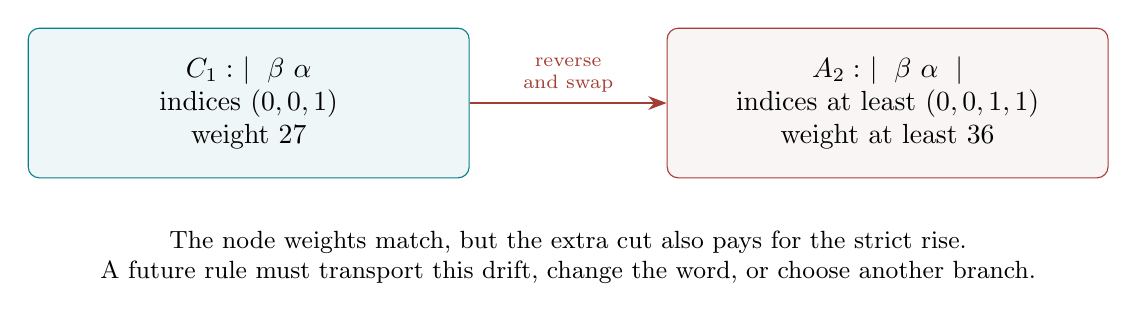
\begin{tikzpicture}[>=Stealth]
\node[draw=teal,fill=pale,rounded corners,minimum width=56mm,minimum height=19mm,align=center] (l)
 {$C_1:\ \mid\ \beta\ \alpha$\\indices $(0,0,1)$\\weight $27$};
\node[draw=warn,fill=warn!5,rounded corners,right=25mm of l,minimum width=56mm,minimum height=19mm,align=center] (r)
 {$A_2:\ \mid\ \beta\ \alpha\ \mid$\\indices at least $(0,0,1,1)$\\weight at least $36$};
\draw[->,thick,warn] (l)--node[above,font=\scriptsize,align=center]{reverse\\and swap}(r);
\node[below=15mm of $(l)!0.5!(r)$,align=center,font=\small]
 {The node weights match, but the extra cut also pays for the strict rise.\\
 A future rule must transport this drift, change the word, or choose another branch.};
\end{tikzpicture}
\caption{An exact obstruction to a specific recurrence recipe.
It does not refute the recurrence or a more flexible bijection.}
\end{figure}

\subsection{The next precise global obligation}

Construct the product-side realization of the $C_n$ row:
\[
\CC_n\longleftrightarrow
\SSA_{n+1}\ \sqcup\
\bigl(\{3n+3\}\times\CC_{n+1}\bigr)\ \sqcup\
\bigl(\{6n+6\}\times\CC_{n+1}\bigr)\ \sqcup\
\bigl(\{6n+8\}\times\SSA_{n+2}\bigr).
\]
Here script letters denote the positive auxiliary objects, not the original
gap class; the singleton notation is a fixed weight shift.
A solution must change more than the cut positions while retaining a fixed
color word: modulo three, the unshifted $A_{n+1}$ branch already requires
the difference between color counts to be divisible by three.
It must also respect the phase change when $n+1$ is divisible by three:
the common tail loses no new part at that step, but one additional terminal
gap becomes locked. These are exact requirements, not evidence that the
needed map exists in any proposed form.

There is also an obstruction to preserving the number of colored particles,
even if colors, indices, and the common tail may otherwise change arbitrarily.
In the $n=0$ row at weight $8$, the $C_0$ object $\beta_0(0)$ together with
one common part $3$ has one colored particle. The other source object is
two copies of $\alpha_0(0)$, each of weight $4$.
The target $A_1$ branch has only a two-particle object at weight $8$;
the shifted $C_1$ branches have none; and the $q^8A_2$ branch has the
zero-particle empty object. Thus no complete realization of this row can
preserve colored-particle count. Cut rotations alone cannot suffice.

\section{A global obstruction to bounded expansion}

The seven possible patterns in a block $\{3j+1,3j+2,3j+3\}$ are
\[
E=\varnothing,\quad A=(1),\quad B=(1,2),\quad C=(1,3),\quad
D=(2),\quad F=(3),\quad G=(3,3).
\]
Every displayed part is translated by $3j$. The successor sets are
\begin{center}
\begin{tabular}{ll}
\toprule
Current state&Allowed next states\\\midrule
$E,A,B,D$&$E,A,B,C,D,F,G$\\
$C,F$&$E,D,F,G$\\
$G$&$E,F,G$\\\bottomrule
\end{tabular}
\end{center}
Checking the boundary pairs and triples proves that this is a complete
encoding, not merely a generating recurrence. The model itself is established
prior work \cite{chernli}.

Let $H$ be its $7\times7$ zero-one adjacency matrix in the listed order.
The positive integer vector
\[
v=(10000,10000,10000,5321,10000,5321,3473)^T
\]
satisfies
\[
H^3v=(1584707,1584707,1584707,843205,1584707,843205,550363)^T
\le159v.
\]
Monotonicity and induction give a bound for \emph{all} powers.
Set $\max\varnothing=0$. For $M\ge0$, padding with empty blocks consequently shows
\begin{equation}\label{eq:gapcount}
\#\{\lambda\in\AA:\max\lambda\le M\}
\le \frac{10000}{3473}\,159^{\lceil M/9\rceil}.
\end{equation}

\begin{theorem}[Maximum-part expansion barrier]\label{thm:entropy}
Let $\BB^*$ be the residue partitions with multiplicities at most seven in
the $1,8$ classes and at most one in the $3,6$ classes. If an injection
$f:\BB^*\to\AA$ satisfies
$\max f(\lambda)\le\gamma\max\lambda+K$ for all inputs, with fixed finite
real $\gamma,K$, then
\[
\gamma\ge\frac{\log256}{\log159}=1.093959803\ldots.
\]
Weight preservation is not required for this obstruction.
\end{theorem}
\begin{proof}
The first $s$ nine-blocks allow $8\cdot2\cdot2\cdot8=256$ choices each,
so there are $256^s$ source objects with maximum at most $9s$.
For $\gamma\ge0$, injectivity and \eqref{eq:gapcount} imply
$256^s\le(10000/3473)159^{\gamma s+K/9+1}$ whenever the maximum bound is
nonnegative. If $\gamma$ is smaller than the stated threshold, the quotient
of the two exponential terms is unbounded. A negative maximum bound is already
impossible. If $\gamma<0$, single-part inputs with unbounded maximum give an
immediate contradiction.
\end{proof}

\begin{figure}[ht]
\centering
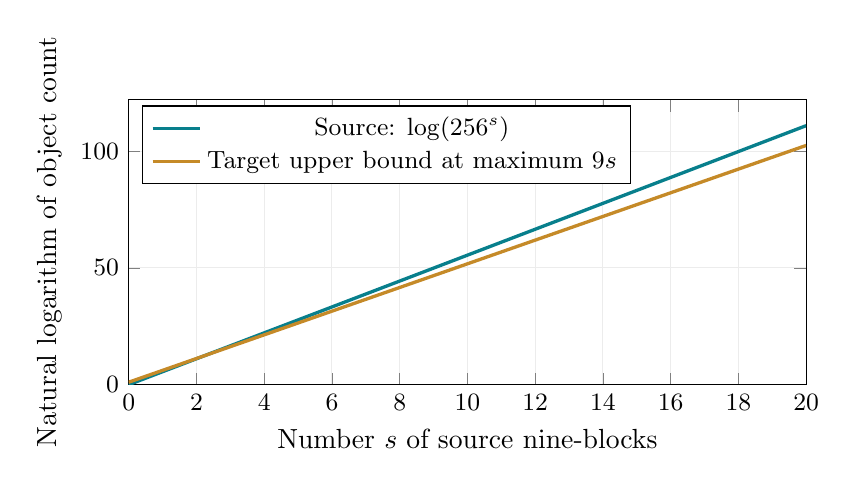
\begin{tikzpicture}
\begin{axis}[width=.84\linewidth,height=5.2cm,xlabel={Number $s$ of source nine-blocks},
ylabel={Natural logarithm of object count},xmin=0,xmax=20,ymin=0,
legend style={at={(0.02,0.98)},anchor=north west,font=\small},
grid=major,grid style={gray!15},tick label style={font=\small}]
\addplot[teal,very thick,domain=0:20,samples=2]{x*ln(256)};
\addlegendentry{Source: $\log(256^s)$}
\addplot[gold,very thick,domain=0:20,samples=2]{ln(10000/3473)+x*ln(159)};
\addlegendentry{Target upper bound at maximum $9s$}
\end{axis}
\end{tikzpicture}
\caption{A slope mismatch survives every fixed additive offset. The theorem
uses a bounded-multiplicity source subset; it is stronger than the immediate
obstruction from arbitrarily many ones.}
\end{figure}

$\BB^*$ is a subset, not a canonical normalization of $\BB$.
The tempting carry $1^8\mapsto8$ collides with the original source $(8)$.
Thus ordinary uncolored Glaisher carrying cannot be invoked to identify
these two source families.

\section{Reversible local surgery and recorded carry failures}

\subsection{A bidegree-preserving switch}

There is a direct local bijection realizing
\begin{equation}\label{eq:switch}
\frac1{(1-x)(1-y)(1-x^2y)}
=\frac1{(1-y)(1-x^2)(1-xy)}
 +\frac{x}{(1-x^2)(1-xy)(1-x^2y)}.
\end{equation}
The input is $(a,b,c)\in\NN^3$, of bidegree
$X=a+2c,\ Y=b+c$. Put
\[
r=X\bmod2,\qquad p=\max\{0,\lfloor(\min(X,Y)-r)/2\rfloor+1\}.
\]
If $c<p$, output the unmarked triple
\[
(d,e,f)=\bigl(Y-r-2c,\ (X-r-2c)/2,\ r+2c\bigr).
\]
Otherwise put $h=(X-1-Y)\bmod2$ and
$g=h+2(c-p)$, and output the marked triple
\[
(e,f,g)=\bigl((X-1-Y-g)/2,\ Y-g,\ g\bigr).
\]
The marker supplies one $x$.

For the inverse, reconstruct $(X,Y)$ from the output, then use
$c=(f-r)/2$ in the unmarked branch or $c=p+(g-h)/2$ in the marked branch.
Finally $a=X-2c$ and $b=Y-c$. At fixed $(X,Y)$, the admissible input
coordinate is the interval $0\le c\le\min(\lfloor X/2\rfloor,Y)$.
The two output arithmetic progressions partition this interval. Splitting
into $Y\ge X$, $Y\le\lfloor X/2\rfloor$, and the intermediate range proves
nonnegativity, coverage, and both inverses, including zero boundaries.
This is fixed integer arithmetic on one local multiplicity coordinate;
it is not a ranking of whole partitions.

The specialization $x=q^{9j+2}$, $y=q^{9k+3}$ maps chosen
residue-$2,3,7$ species to residue-$3,4,5$ species or a marked alternative.
To compose switches globally one must still recover $j,k$, branch labels,
and shared-species context. These are not supplied by \eqref{eq:switch}.
The full formulas and the separate interval-proof review are in the supplement.

\subsection{A reversible carry that exposes the missing information}

For a part $s\equiv\pm1\pmod9$, write its multiplicity
$m_s=4q_s+2d_s+e_s$, where $d_s,e_s\in\{0,1\}$.
Replace it by $e_s$ copies of $s$, $d_s$ copies of $2s$, and $q_s$ copies
of $4s$; leave the $\pm3$ classes unchanged. The four residue lanes
$\pm1,\pm2,\pm4,\pm3$ are disjoint, so division by $1,2,4$ recovers the
parent species. This is a total weight-preserving auxiliary bijection.
It does not produce the gap class: $1^8$ becomes $(4,4)$.

\begin{center}
\begin{tabularx}{\linewidth}{lXX}
\toprule
Proposed repair&Two distinct source inputs&Shared output or failure\\\midrule
$(4s,4s)\mapsto8s$&$1^8$ and $(8)$&$(8)$\\
$(4s,4s)\mapsto(s,7s)$&$10^8$ and $(10,35,35)$&$(10,70)$\\
$(4s,4s)\mapsto(2s,6s)$&$1^8$ and $(1,1,6)$&$(2,6)$\\
$(4s,4s)\mapsto(3s,5s)$&$8^8$ and $(10,10,10,10,24)$&$(24,40)$\\
Leave $(4s,4s)$&$1^8$&Invalid close pair $(4,4)$\\\bottomrule
\end{tabularx}
\end{center}
The collisions assume the other lanes are unchanged and uncolored.
They do not exclude context-dependent coordinated repairs.

One origin-preserving alternative is the involution
\[
(m_s,m_{rs})=(rq+d,b)\longmapsto(rb+d,q),\qquad 0\le d<r.
\]
It preserves $m_s+rm_{rs}$ and exchanges the quotient with the neighboring
multiplicity. Applying it to disjoint $8$-adic pairs in the $\pm1$ lanes and
$2$-adic pairs in the $\pm3$ lanes gives a total involution of the source.
It retains information but does not normalize every lower digit. On two
species alone, such a normalization is impossible: $(r,0)$ and $(0,1)$
would have only one normalized target of weight $rs$.

\section{Formal assurance, reproduction, and preserved failures}

\subsection{What Lean actually checks}

The four standalone modules use \texttt{import Std} with Lean
\texttt{4.34.0}. Each was freshly compiled; the verification record contains
the exact source hashes, commands, exit codes, and printed axiom reports.
No reported theorem uses \texttt{sorryAx} or an added axiom.
Standard foundational axioms are reported explicitly rather than described
as an axiom-free development.

\begin{center}
\begin{tabularx}{\linewidth}{lXX}
\toprule
Module&Universally checked content&Boundary of the certificate\\\midrule
\texttt{Cancellation.lean}&Least-eligible involution on arbitrary finite lists;
weight, sign parity, exact fixed points&Does not formalize divided differences,
cut flattening, or the full KR1 map\\
\texttt{Blocks.lean}&Seven-state multiplicity classification, transitions,
existence and uniqueness of compatible sequences&Sorted partition lists,
finite support and weight translation remain written arguments\\
\texttt{Entropy.lean}&Integer matrix witness and path bound for every power&
Source counting, partition encoding and logarithmic limit remain written\\
\texttt{MergeBounds.lean}&Boundary identities and the nonadjacent selection
inequalities for the cluster merge&Does not verify the entire merge algorithm\\\bottomrule
\end{tabularx}
\end{center}

The central formal signatures include
\begin{verbatim}
cancel_involution : cancel (cancel xs) = xs
cancel_weight    : weight start (cancel xs) = weight start xs
cancel_parity    : hasEligible xs = true ->
                   parity (cancel xs) = !(parity xs)
fixed_iff_all_zero :
  cancel xs = xs <-> forall x in xs, x = (false, 0)
walks_bound : walks n s <= 159^n * v s
\end{verbatim}
These are readable renderings; the exact checked Lean declarations are supplied.

\subsection{Independent checks and reviews}

The positive-word construction was checked against the primary cut expansion
by a distinct agent. A second implementation tested $3{,}178{,}008$ bounded
cut-word states for $n=3,4,6$; an independently written test checked
$124{,}944$ states for $n=3,6$. Both checked coordinate recovery, the
involution, sign, weight, and survivors. The local surgery test covered
$27{,}000$ input triples and bounded boxes in both output branches.
The lane and paired-carry checks covered $5{,}461$ source objects through
weight $40$. These numbers describe finite checks, not proof coverage.

Separate reviews support the existing direct cluster merge and the new local
constructions. The previous $a\le2$ formulas were briefly rediscovered, then
recognized as already present in RR003 and removed from the contribution list.
A contradictory draft sentence about the height-block mask $\{3\}$ was corrected.
The failed uncolored Glaisher normalization, sequential marker cancellation,
and layer-reversal proposals remain in the failure ledger.

\subsection{Run the supplement}

The accompanying package preserves the new mathematical notes, four Lean files,
exact checks, source-bound reviews, and a reproduction script. Run
\begin{verbatim}
python3 verify.py --lean /path/to/lean
pdflatex -interaction=nonstopmode -halt-on-error kr1-positive-models.tex
pdflatex -interaction=nonstopmode -halt-on-error kr1-positive-models.tex
\end{verbatim}
The complete research archive also contains the historical regression context.
The article and its illustrations are generated from this LaTeX source.

\section{Research judgement and next theorem}

The main useful change is global in the auxiliary parameter: the signed
product states now have explicit positive objects for every $n$.
That resolves a real obstacle which first appears at $n=3$, and it works
simultaneously for all residual markers. It is broader than a new restricted
KR1 subfamily, but it is still an intermediate construction.

The intuition behind the successful step was to change coordinates before
adding more cases. A marker of weight $9h$ should act on an actual suffix of
$h$ objects, not on an arbitrarily chosen particle. Flattening identifies that
suffix intrinsically, including cuts. The failed attempts identify what a
future recurrence must retain: origin information in carries, layer labels at
equal cuts, the forced-descent weight, and the phase of $n$ modulo three.

The next decisive target is the explicit four-branch correspondence in
Section~\ref{sec:gap}, followed by the other two matrix rows and a terminating
boundary argument. A proposed map should first meet the weight-$27$ versus
$36$ witness, the occupied shared-boundary cases, and the phase where an
additional terminal gap is locked. Increasing the size of a finite apex
table would not meet those obligations.

\statusbox{\textbf{Final claim boundary.}
Proved here: a general positive normalized divided-difference model,
all-index positive KR auxiliary models, specified local bijections and
obstructions, with scoped Lean certificates and independent reviews.
Not proved here: an explicit structural bijection
$\BB_N\leftrightarrow\AA_N$ for every $N$.
No percentage of the open problem being solved is assigned.}

\appendix
\section{The audited gap-to-cluster endpoint}

Every close pair is
$P_{2r}=(3r+1,3r+2)$ or $P_{2r+1}=(3r+3,3r+3)$.
Close pairs cannot overlap. Splitting a gap partition into these pair atoms
and the remaining singles gives the boundary functions
\[
\begin{array}{c|cc}
&L(\ell)&R(\ell)\\\hline
\ell=2r&3r-1&3r+4\\
\ell=2r+1&3r&3r+6
\end{array}
\]
A single before $P_\ell$ must be at most $L(\ell)$; one after it must be
at least $R(\ell)$. Successive pairs require a level difference of at least two.
The key identity is $R(\ell)-3=L(\ell+1)+1$.

For single $s_i$ with $i$ earlier singles and $q_i$ earlier pairs, and pair
$P_{\ell_j}$ with $j$ earlier pairs and $z_j$ earlier singles, define
\[
\mu_i=s_i-3q_i-2i-1,\qquad
\nu_j=\ell_j-2j-z_j.
\]
The boundary inequalities imply nonnegative increasing coordinate lists.
Conversely, after emitting $i$ singles and $j$ pairs, compare
$S=\mu_i+3j+2i+1$ and $\ell=\nu_j+2j+i$.
Emit the single exactly when $S\le L(\ell+1)$; otherwise emit $P_\ell$.
An exhausted list leaves the other type.

For nonadjacent competing atoms, the same threshold follows by bounding the
intervening singles by steps of two, or the intervening pair levels by steps
of two. These are the inequalities checked in \texttt{MergeBounds.lean}.
Extraction and merging recover each coordinate and each atom, hence are
mutually inverse. Finally,
$\sum_iq_i+\sum_jz_j=ab$, since each single-pair combination has one order.
Summing the coordinates gives
\[
|\lambda|=a^2+3ab+3b^2+|\mu|+3|\nu|.
\]
The existing repository proof of this endpoint received a fresh independent
semantic review during this investigation. The source theorem and cluster
idea are attributed to Kur\c{s}ung\"oz; this endpoint does not supply the missing
residue-to-cluster map.

\begin{thebibliography}{9}
\bibitem{xia}
E.\ X.\ W.\ Xia, \emph{The modulo 9 Kanade--Russell identities and their
Nahm-sum duals}, arXiv:2609.08816v1 (2026).
\url{https://arxiv.org/html/2609.08816v1}.
Inspected: Lemma 2.2 and the auxiliary definitions and recurrences in Sections 3--4.
\bibitem{mizuno}
Y.\ Mizuno, \emph{The three Kanade--Russell identities modulo nine},
arXiv:2609.09653 (2026).
\url{https://arxiv.org/abs/2609.09653}.
\bibitem{palomar}
Y.\ Mizuno, \emph{KR-mod9-lean}, Palomar record
PALOMAR-2026-09-10-000002, version 1.
\url{https://palomar-registry.org/entry?id=PALOMAR-2026-09-10-000002&version=1}.
Pinned source \texttt{d8b921339ecc}; registry-reported verification, not a local rerun.
\bibitem{kursungoz}
K.\ Kur\c{s}ung\"oz, \emph{Andrews--Gordon type series for Kanade--Russell
conjectures}, arXiv:1808.01432, Theorem 7.
\url{https://arxiv.org/abs/1808.01432}.
\bibitem{chernli}
S.\ Chern and Z.\ Li, \emph{Linked partition ideals and Kanade--Russell
conjectures}, Discrete Mathematics 343 (2020), 111876.
\url{https://arxiv.org/abs/1809.08655}.
\bibitem{andrewskeith}
G.\ E.\ Andrews and W.\ J.\ Keith, \emph{Schmidt-type theorems for partitions
with uncounted parts}, arXiv:2203.05202v2, Section 2 and Theorem 6.
\url{https://arxiv.org/abs/2203.05202}.
\bibitem{repo15}
C.\ Yamba and contributors, \emph{Phase 2: corrected tableau injections,
beta recovery and bounded KR1 octant evidence}, Yamba AI Math PR \#15.
\url{https://github.com/cyamba/yamba-ai-math/pull/15}.
\bibitem{repo16}
C.\ Yamba and contributors, \emph{Argon continuation: cone classification,
all-parameter a3b0 proof and compiler obstruction}, Yamba AI Math PR \#16.
\url{https://github.com/cyamba/yamba-ai-math/pull/16}.
\end{thebibliography}
\end{document}
